\documentclass[utf8]{ctexart}
\usepackage{graphicx}
\usepackage{amsmath,amssymb,amsthm}
\usepackage{geometry}
\usepackage{enumitem}
\usepackage{xcolor}
\usepackage{mdframed}
\usepackage{tikz}
\usepackage{booktabs,array}
\usepackage{needspace}
\usepackage[hidelinks]{hyperref}
\usetikzlibrary{arrows.meta,positioning,calc}
\geometry{a4paper,margin=2.5cm}

\newtheoremstyle{mystyle}
  {8pt}{8pt}{\kaishu}{0pt}{\bfseries}{}{1em}{}
\theoremstyle{mystyle}
\newtheorem{theorem}{定理}
\newtheorem{lemma}{引理}

\title{\textbf{人工智能导论\quad 第一次作业}}
\date{\today}
\author{李子嘉 2024012325}

\begin{document}
\maketitle

\section*{题目1}
\textbf{证明：}

当终点 $T$ 即将从边缘集（frontier）中取出时，树搜索的边缘集中仍有
最优路径上的某个节点 $n^*$，其对应路径为该最优路径的前缀，因而
\[
  g(n^*)+h^*(n^*)=h^*(S).
\]
由于 $T$ 的 $f$ 值最小，且 $h(T)=0$，故
\[
  g(T)=f(T)\le f(n^*)=g(n^*)+h(n^*).
\]

\subsection*{（1）}
代入 $h(n^*)\le h^*(n^*)+C_1$，得到
\[
  g(T)\le g(n^*)+h^*(n^*)+C_1=h^*(S)+C_1.
\]

\subsection*{（2）}
由边代价非负可知 $g(n^*)\ge0$，又有 $C_2\ge1$，因此
\begin{align*}
  g(T)
  &\le g(n^*)+C_2h^*(n^*)\\
  &\le C_2\bigl(g(n^*)+h^*(n^*)\bigr)
   =C_2h^*(S).
\end{align*}

\newpage
\subsection*{（3）}
记最优代价为 $C^*=h^*(S)$，返回解的代价为 $C=g(T)$。
这里先考虑不重新打开 CLOSED 节点的图搜索，仍更新 OPEN 中的更优路径，
按 $g+h$ 取出节点，并在取出终点时停止。

\medskip
\noindent\textbf{先检查不高估的情形。}
看到“类似的结论”，我首先想到沿用前两问的条件。但不妨先令 $C_1=0$
或 $C_2=1$：此时条件都是 $h\le h^*$，结论都应当退化为 $C=C^*$。
而我们知道，不重新打开节点的图搜索仅靠不高估并不能保证最优，
还可能因为不一致的启发函数过早关闭节点。因此，我们猜测这种直接推广并不成立，
并用下面的例子确认这一点：
\begin{center}
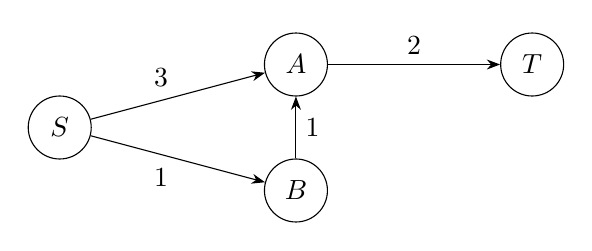
\begin{tikzpicture}[
  >=Stealth,
  vertex/.style={circle,draw,minimum size=8mm,inner sep=0pt},
  every edge/.style={draw,->},
  every edge quotes/.style={fill=white}
]
  \node[vertex] (S) at (0,0) {$S$};
  \node[vertex] (A) at (3,0.8) {$A$};
  \node[vertex] (B) at (3,-0.8) {$B$};
  \node[vertex] (T) at (6,0.8) {$T$};
  \draw[->] (S) -- node[above left] {$3$} (A);
  \draw[->] (S) -- node[below left] {$1$} (B);
  \draw[->] (B) -- node[right] {$1$} (A);
  \draw[->] (A) -- node[above] {$2$} (T);
\end{tikzpicture}
\end{center}
按 $S,A,B,T$ 的顺序取
\[
 (h(S),h(A),h(B),h(T))=(4,0,3,0),\qquad
 (h^*(S),h^*(A),h^*(B),h^*(T))=(4,2,3,0).
\]
扩展 $S$ 后，$f(A)=3<f(B)=4$，所以先关闭 $A$，生成 $g(T)=5$。
随后扩展 $B$，发现代价为 $2$ 的路径 $S\to B\to A$，但不再打开 $A$，
最终返回 $C=5$；最优路径 $S\to B\to A\to T$ 的代价却是 $C^*=4$。
这里所有节点均满足 $h\le h^*$，但 $h(B)=3>1+h(A)$，违反了一致性。

这说明连不高估的基准情形都不能保证最优，因而已经没有必要再尝试证明
原条件对一般 $C_1,C_2$ 的机械推广。联想到图搜索的问题并不只是启发函数是否高估，而在于 CLOSED 节点不再打开，因此更自然的量是启发函数违反一致性的程度。于是我们思考：
\textbf{如果放宽的是一致性条件，能否得到类似的误差控制？}

\medskip
\noindent\textbf{带着这个问题查阅文献。}
我们检索后发现，Valenzano 等人\cite{valenzano2014}恰好研究了不重新展开节点时的
解质量损失。以下按文献取有限图、有限非负启发函数、非负边代价及 $h(T)=0$，
用每条边对一致性条件的违反程度
\[
 I(u,v)=\max\{h(u)-c(u,v)-h(v),\,0\}.
\]
来度量误差。设 $P^*=(n_0=S,n_1,\ldots,n_k=T)$ 为最优路径，$k\ge1$，
该文定理 4.6 给出
\begin{equation}
 \boxed{C\le C^*+\sum_{j=1}^{k-1}I(n_j,n_{j+1}).}
 \label{eq:inconsistency-bound}
\end{equation}
这个结论不要求 $h$ 不高估。求和不含首边，因为 $S$ 首先以正确的 $g(S)=0$
扩展，最优路径上的 $n_1$ 会获得正确的前缀代价。

为了看清它与前两问的联系，我们整理证明的关键步骤。在取出 $T$ 前，选 $P^*$ 上最靠近起点的
OPEN 节点 $n_i$，则
\[
 C\le f(n_i)
 =C^*+\underbrace{g(n_i)-g^*(n_i)}_{\text{前缀代价误差}}
       +\underbrace{h(n_i)-h^*(n_i)}_{\text{启发估计误差}}.
\]
文献的定理 4.5 及其对该 OPEN 节点的推论给出前缀误差界；
后缀误差界则由 $h(n_j)-h(n_{j+1})-c(n_j,n_{j+1})\le I(n_j,n_{j+1})$
沿后缀求和得到：
\[
 g(n_i)-g^*(n_i)\le\sum_{j=1}^{i-1}I(n_j,n_{j+1}),\qquad
 h(n_i)-h^*(n_i)\le\sum_{j=i}^{k-1}I(n_j,n_{j+1}).
\]
两式相加即得式\eqref{eq:inconsistency-bound}。相比前两问，这里多出的 $g$ 值误差
也由不一致量控制，其中前缀误差的归纳结论引用自文献。

\newpage
\noindent\textbf{回到本题，尝试给出相应的条件。}
有了式\eqref{eq:inconsistency-bound}，我们就可以从一致性出发，分别尝试加法和乘法放宽，
并直接证明与前两问对应的结论。
\begin{enumerate}[label=\arabic*.,leftmargin=2em,itemsep=8pt]
 \item \textbf{加法放宽：}
 若每条边都有 $h(u)\le c(u,v)+h(v)+\delta$，其中 $\delta\ge0$，则
 \[
   I(u,v)\le\delta
   \quad\Longrightarrow\quad C\le C^*+(k-1)\delta.
 \]
 若已知最优路径至多有 $D$ 条边，则可用 $(D-1)\delta$ 作统一加法误差界。
 与第（1）问不同，每条边的放宽量会累积；若希望仍保证 $C\le C^*+C_1$，
 一个充分条件是最优路径上除首边外的不一致量之和不超过 $C_1$。

 \item \textbf{乘法放宽：}
 若每条边都有 $h(u)\le w\,c(u,v)+h(v)$，其中 $w\ge1$，则
 \[
   I(u,v)\le(w-1)c(u,v),
   \qquad
   C\le C^*+(w-1)\sum_{j=1}^{k-1}c(n_j,n_{j+1})\le wC^*.
 \]
 取 $w=C_2$ 就得到与第（2）问相同形式的界，但条件从点上的
 $h\le C_2h^*$ 加强为每条边上的不等式。
\end{enumerate}

\medskip
\noindent\textbf{结论}
所以图搜索确实存在与前两问类似的误差界，但需要控制的是一致性误差而不是单个节点上的高估误差，且加法放宽的程度与最优路径的长度有关，不好控制。若允许重新打开 CLOSED 节点，则原来的 admissibility 型条件又可以得到相应的界。

\begingroup
\small
\begin{thebibliography}{9}
\bibitem{valenzano2014}
R. Valenzano, N. R. Sturtevant, and J. Schaeffer.
\href{https://www.cs.du.edu/~sturtevant/papers/non_reopening.pdf}
{Worst-Case Solution Quality Analysis When Not Re-Expanding Nodes in Best-First Search}.
AAAI, 2014. 第 4.1--4.3 节，尤其定理 4.5、4.6。
\end{thebibliography}
\endgroup

\clearpage
\section*{题目2}
\markboth{题目2}{题目2}
计分部分已全部通过（52/52），结果如下。
\begin{center}
  
\includegraphics[width=\textwidth]{figures/calculation-passed.png}
\end{center}

\medskip
\noindent\textbf{关于出题的一点观察。}
做完后，我发现模拟退火一直在附近往返，遗传算法的子代甚至变回了父代，
于是检查了随作业提供的 \texttt{code/calculation/generator.py}。

\medskip
\noindent\textbf{模拟退火：覆盖了分支，却没有展示出优化效果。}
生成器确实要求出现接受劣解、拒绝劣解和接受更优候选的情况，
还排除了容易受小数舍入影响的概率比较。但我的轨迹是
\[
 F(4)\to G(6)\to F(4)\to G(6)\to G(6)\to G(6)\to H(7),
\]
而爬山法直接得到 $F(4)\to E(10)\to D(17)$。
这条轨迹满足了所有筛选条件，却主要在 $F,G$ 之间往返：
可以说，出题条件被这种退化轨迹“钻了空子”。它能练习接受概率的计算，
但就展示“接受暂时变差以逃离局部最优”而言，几乎没有起到作用。
当然，短程退火本来就不保证优于爬山；我的建议是增加一类跨越低谷、
到达更好局部峰的示例，使计算规则与算法动机联系起来。

\medskip
\noindent\textbf{轮盘赌：低适应度个体也有机会。}
一个有意思的细节是，生成器先等概率抽取两个不同的轮盘区间，
再在各区间内部生成随机数，并避开边界。因此，题面上的选择结果仍符合
轮盘赌规则，但跨题统计时，父代的出现频率并不等于适应度占比。
我觉得这一安排有很好的教学意义：它让不同适应度的个体都有机会出现在例题中，
尤其能提醒我们，轮盘赌并非只选择适应度最高的个体，低适应度也可以被选上。

\clearpage
\noindent\textbf{遗传操作：建议避免交叉与变异完全抵消。}
我的两个父代、交叉结果与变异结果依次为
\begin{center}
\begin{tabular}{lll}
\toprule
阶段 & 个体1 & 个体2\\
\midrule
父代 & \texttt{001110}（P4） & \texttt{101111}（P2）\\
第3位后交叉 & \texttt{001111} & \texttt{101110}\\
反转第6位 & \texttt{001110}（P4） & \texttt{101111}（P2）\\
\bottomrule
\end{tabular}
\end{center}
两个后缀仅末位不同，交换后再翻转末位，恰好分别回到原父代。
判分检查发现这不是计算错误，但在仅展示一代操作的题目里，确实有点“忙了一圈回到原点”。
建议生成器过滤这种完全抵消的情况，或明确把它作为讨论遗传操作不保证改进的反例。

为检查这是否只是个例，我们复现了整数种子 $0,\ldots,999$ 的题组。
其中，两个变异子代均属于初始种群的有 $36$ 组（$3.6\%$），
但与我这题一样、两个子代\emph{分别恢复为所选原父代}的只有 $10$ 组（$1.0\%$）。

为了确认事件并非故意按排，我还检查了学号如何映射到随机数生成器的种子。结果显示，代码先去掉学号两端空白，将字符串
\texttt{AI2026-search:} 与学号拼接后做 SHA-256，
取摘要前 $8$ 字节，按大端序解释为 $64$ 位非负整数，
再交给 \texttt{random.Random(seed)}。因此并不是对学号取模；
相邻学号也不会对应相邻种子，学号已被打散。

于是我们将
\texttt{2024012000} 至 \texttt{2024012999} 这 $1000$ 个\emph{模拟学号}
经过实际哈希流程后再生成题目，以上两个事件分别出现 $27$ 次（$2.7\%$）
和 $9$ 次（$0.9\%$）。虽然这仍不是课程名单的统计，但也说明了我这个学号的情况并非刻意安排，而是小概率随机事件发生在我身上，并建议改善样例筛选。

% 完成最终报告时，请自行调整文字，并按题面要求在末尾声明大模型辅助的方式和程度。（帮助查阅第一题第三问的开放式问题相关文献并总结定理证明）

\clearpage
\section*{题目3}
\markboth{题目3}{题目3}
\subsection*{（1）（2）实现与验证}
回溯搜索在合法填数后递归，并在返回时恢复空格，最终枚举得到 $288$ 个互不相同的合法解。
局部搜索保持每行是 $1,2,3,4$ 的排列，从冲突格中随机选取一个，
评估三个同行交换，并随机执行其中总冲突最少的一项。同列与同宫重叠的冲突只计一次。
两份随作业提供的测试文件共 $8$ 项测试全部通过。

用种子 $0,\ldots,999$ 运行局部搜索，$1000$ 次均成功且未发生重启；
实际交换次数平均为 $6.221$，中位数为 $5$，第 $95$ 百分位为 $13$，最大为 $32$。
这里一次交换包含选择、评估和执行三个可视化事件，不能把界面的前进次数直接当成交换次数。

\subsection*{（3）其他求解方法与尝试}
\noindent\textbf{局部搜索并不只有题目给出的这一种。}
我首先对局部搜索的具体算法进行了扩展尝试。题目中将冲突数最少的交换作为候选执行，但类似模拟退火的思想，我们也可以允许随机选择的较差交换被接受，从而有机会离开局部极小值。
例如仍然只交换同行数字，但以总冲突数 $E$ 为目标使用模拟退火：
随机选一行及其中两个不同位置，交换后若 $\Delta E\le0$ 就接受，否则以
$\exp(-\Delta E/T)$ 的概率接受；逐渐降低温度，遇到 $E=0$ 即找到解。

\medskip
\noindent\textbf{约束传播与启发式回溯。}
若考虑回溯搜索的启发式改进，我们可以联想起人类解数独的思路：先确认哪些格子只有一个候选数字，填入后继续传播约束，直到没有单候选格子为止。此时再执行回溯搜索。候选为空就立即回溯；仍需分支时，优先选择候选最少的格子（MRV）。填入后重新计算候选，继续传播约束。它利用当前约束来决定搜索顺序，而不是始终选择按行扫描遇到的第一个空格。继续遍历所有分支仍可枚举全部解。

\medskip
\noindent\textbf{算法对比}
我在独立的 \texttt{experiments/sudoku\_benchmark.py} 中实现了上述方法，
保留已完成的作业代码作为 baseline。局部搜索对比采用相同的 $1000$ 个种子，
并逐次检查两个方法的初始棋盘完全一致；每轮上限为 $1000$ 次迭代，最多重启 $20$ 次。
退火采用 $T_t=2(0.05/2)^{t/999}$（$t=0,\ldots,999$），每次重启重新降温，
参数预先固定，未按这些种子的结果调优。
所有返回棋盘都通过独立的行、列、宫合法性检查。
\begin{center}
\begin{tabular}{lrr}
\toprule
指标 & 本题最小冲突 & 模拟退火\\
\midrule
成功次数 & $1000/1000$ & $1000/1000$\\
平均迭代次数 & $6.221$ & $114.372$\\
平均实际交换次数 & $6.221$ & $64.117$\\
平均总冲突函数调用次数 & $25.884$ & $115.372$\\
单次用时中位数（毫秒） & $0.334$ & $1.268$\\
\bottomrule
\end{tabular}
\end{center}
一次 baseline 迭代评估三个候选并执行一个，而退火一次迭代只提出一个候选且可能拒绝，
所以迭代次数不能直接视作等量计算。表中同时记录了目标函数调用和实际用时。完整逐次记录保存在
\texttt{experiments/results/sudoku\_runs.csv}。

\textbf{本次实验并没有支持“更复杂就更好”。}
这组空 $4\times4$ 棋盘上，最小冲突法已经很有效，模拟退火反而多走了许多步。
这只能说明所选退火参数与邻域策略在这个小问题上不占优势，与先前计算题退火的表现相似。
回溯对比则单独以“枚举所有解”为任务，
两种回溯方法得到的解集合完全相同，均为 $288$ 个；各重复 $30$ 次，
原实现用时中位数为 $8.260$ 毫秒，MRV 版本为 $15.213$ 毫秒。
候选集合维护也有成本，在这个小而对称的问题上也没有体现出速度收益。

\medskip
\noindent\textbf{遗传算法的讨论：}

我的第一反应是，数独有着全局约束，两个好棋盘拼起来，并不保证生成更好的棋盘。数独的约束跨越多个位置，单个数字脱离所在行、列和宫格，
并没有独立的“优良基因”含义。甚至两个完全合法的解交叉，也可能产生不合法子代。
例如下面两个父代都是合法解：
\[
 A=\begin{pmatrix}1&2&3&4\\3&4&1&2\\2&1&4&3\\4&3&2&1\end{pmatrix},
 \qquad
 B=\begin{pmatrix}2&1&3&4\\3&4&2&1\\1&2&4&3\\4&3&1&2\end{pmatrix}.
\]
取 $A$ 的前两行和 $B$ 的后两行，子代第一列变成 $(1,3,1,4)$，出现重复。
因此，交叉不保证降低冲突，甚至不保证保留父代已有的合法性。

虽然这并不意味着遗传算法无法用于数独，需要设计完善的表示和操作或许可用，但
对于这个小问题，遗传算法的优势显然并不明显。

\medskip
\noindent\textbf{大模型辅助说明（截至本题）：}
第一题使用大模型辅助检索文献、梳理定理及整理表述；第二题使用大模型辅助检查出题代码、
统计样例并整理反馈；第三题的作业回溯与最小冲突代码由本人完成，
使用大模型辅助检查代码，并编写独立对比实验、运行验证和整理本节文字。

\end{document}
